\documentclass{beamer}

\usepackage[utf8]{inputenc}
\usetheme{Madrid}
\usecolortheme{seahorse}

\title{Pengantar Arsitektur Perusahaan}
\author{Alfa Yohannis}
\date{\today}

\begin{document}
	
	\frame{\titlepage}
	
	\begin{frame}
		\frametitle{Definisi 'Enterprise' Menurut Oxford English Dictionary}
		\begin{itemize}
			\item Sebuah proyek atau usaha, biasanya satu yang membutuhkan upaya dan keberanian.
			\item Inisiatif, berani mengambil risiko dalam harapan mendapatkan keuntungan.
			\item Organisasi atau perusahaan bisnis.
		\end{itemize}
	\end{frame}
	
	\begin{frame}
		\frametitle{Definisi 'Enterprise' Menurut Cambridge English Dictionary}
		\begin{itemize}
			\item Kemampuan untuk berpikir tentang rencana baru dan membuat mereka berhasil.
			\item Sebuah perusahaan.
		\end{itemize}
	\end{frame}
	
	\begin{frame}
		\frametitle{Definisi 'Enterprise' Menurut Merriam-Webster Dictionary}
		\begin{itemize}
			\item Sebuah proyek atau usaha yang seringkali memerlukan keberanian.
			\item Kesiapan untuk terlibat dalam usaha yang berani dan berisiko.
			\item Sebuah unit ekonomi terorganisir.
		\end{itemize}
	\end{frame}
	
	\begin{frame}
		\frametitle{Kesimpulan Definisi `Enterprise'}
		\begin{itemize}
			\item 'Enterprise' biasanya merujuk pada proyek atau usaha yang berani dan berisiko.
			\item Dapat juga merujuk pada sebuah organisasi atau perusahaan bisnis.
			\item Definisi ini umumnya konsisten di antara berbagai kamus Bahasa Inggris terkemuka.
		\end{itemize}
	\end{frame}
	
	\begin{frame}
		\frametitle{Definisi 'Architecture' Menurut Oxford English Dictionary}
		\begin{itemize}
			\item Seni atau praktek merancang dan membangun bangunan.
			\item Gaya atau metode konstruksi.
			\item Susunan atau struktur sesuatu.
		\end{itemize}
	\end{frame}
	
	\begin{frame}
		\frametitle{Definisi 'Architecture' Menurut Cambridge English Dictionary}
		\begin{itemize}
			\item Seni dan praktek merancang bangunan.
			\item Gaya atau desain bangunan khusus atau sekelompok bangunan.
			\item Cara yang dilakukan atau disusun sesuatu.
		\end{itemize}
	\end{frame}
	
	\begin{frame}
		\frametitle{Definisi 'Architecture' Menurut Merriam-Webster Dictionary}
		\begin{itemize}
			\item Seni atau ilmu merancang dan membangun bangunan.
			\item Metode atau gaya konstruksi.
			\item Cara bagaimana bagian-bagian dari sesuatu disusun atau disistematisasi.
		\end{itemize}
	\end{frame}
	
	\begin{frame}
		\frametitle{Ringkasan}
		\begin{itemize}
			\item 'Architecture' umumnya merujuk pada seni atau praktek merancang dan membangun bangunan.
			\item Dapat juga merujuk pada gaya atau metode konstruksi.
			\item Selain itu, juga dapat merujuk pada cara bagian-bagian dari sesuatu disusun atau disistematisasi.
		\end{itemize}
	\end{frame}
	
	\begin{frame}
		\frametitle{Definisi Arsitektur menurut IEEE}
		\begin{itemize}
			\item Organisasi fundamental dari suatu sistem
			\item Melibatkan komponen sistem, hubungan antar komponen
			\item Mengatur desain dan evolusi sistem
			\item Komponen sistem dapat mencakup perangkat keras, perangkat lunak, data, manusia, proses
		\end{itemize}
	\end{frame}
	
	
	
	\begin{frame}
		\frametitle{Definisi 'Enterprise Architecture' Menurut Gartner}
		\begin{itemize}
			\item Sebuah disiplin untuk proyek desain, perencanaan, implementasi, dan kontrol.
			\item Membantu organisasi mencapai konsistensi bisnis dan IT.
			\item Melibatkan kerjasama antara berbagai stakeholder.
			\item Dapat digunakan untuk membantu dalam pengambilan keputusan strategis.
		\end{itemize}
	\end{frame}
	
	\begin{frame}
		\frametitle{Definisi 'Enterprise Architecture' Menurut TOGAF}
		\begin{itemize}
			\item Sebuah kerangka kerja arsitektur.
			\item Menyediakan definisi dan desain dasar untuk arsitektur perusahaan.
			\item Membantu memastikan operasi perusahaan berjalan secara konsisten dan efisien.
			\item Berfokus pada standar dan prosedur yang digunakan dalam perusahaan.
		\end{itemize}
	\end{frame}
	
	\begin{frame}
		\frametitle{Definisi 'Enterprise Architecture' Menurut ISO/IEC/IEEE 42010}
		\begin{itemize}
			\item Pendekatan fundamental terhadap organisasi suatu sistem.
			\item Melibatkan pemahaman semua komponen, hubungan antar komponen, dan lingkungan mereka.
			\item Menekankan pentingnya struktur dan interaksi dalam sistem.
			\item Menyediakan kerangka kerja untuk pemahaman dan desain sistem.
		\end{itemize}
	\end{frame}
	
	
	\begin{frame}
		\frametitle{Berbagai Kerangka Kerja Arsitektur Enterprise}
		\begin{itemize}
			\item Business System Planning (BSP)
			\item PRISM Architecture Framework
			\item NIST Enterprise Architecture Model
			\item Zachman Framework
			\item EAP: Enterprise Architecture Planning
			\item Sherwood Applied Business Security Architecture
			\item Federal Enterprise Architecture Framework
			\item Gartner’s Enterprise Architecture Method
			\item Department of Defence Architecture Framework (DoDAF)
			\item Australian Government AGA
			\item Business Architecture Body of Knowledge (BizBoK)
			\item ISO Standard for Enterprise Modelling (ISO19439)
		\end{itemize}
	\end{frame}
	
	\begin{frame}
		\frametitle{Perencanaan Sistem Bisnis}
		\begin{itemize}
			\item Perencanaan Sistem Bisnis (Business System Planning/BSP) adalah proses untuk mengidentifikasi, memodelkan, dan menyesuaikan proses bisnis dan sistem informasi dengan tujuan strategis organisasi.
			\item BSP membantu organisasi dalam mengevaluasi proses bisnis yang ada, mengidentifikasi area perbaikan, dan merancang keadaan masa depan sistem bisnis.
			\item Proses ini melibatkan pemahaman terhadap tujuan bisnis, analisis proses bisnis, dan merancang arsitektur sistem informasi yang mendukung proses-proses tersebut.
			\item BSP membantu organisasi meningkatkan efisiensi, menyederhanakan operasi, dan mengoptimalkan alokasi sumber daya.
		\end{itemize}
	\end{frame}
	
	{
		\setbeamertemplate{navigation symbols}{}
		\setbeamertemplate{footline}{}		
		\begin{frame}
			\frametitle{Business System Planning (BSP)}
			\begin{center}
				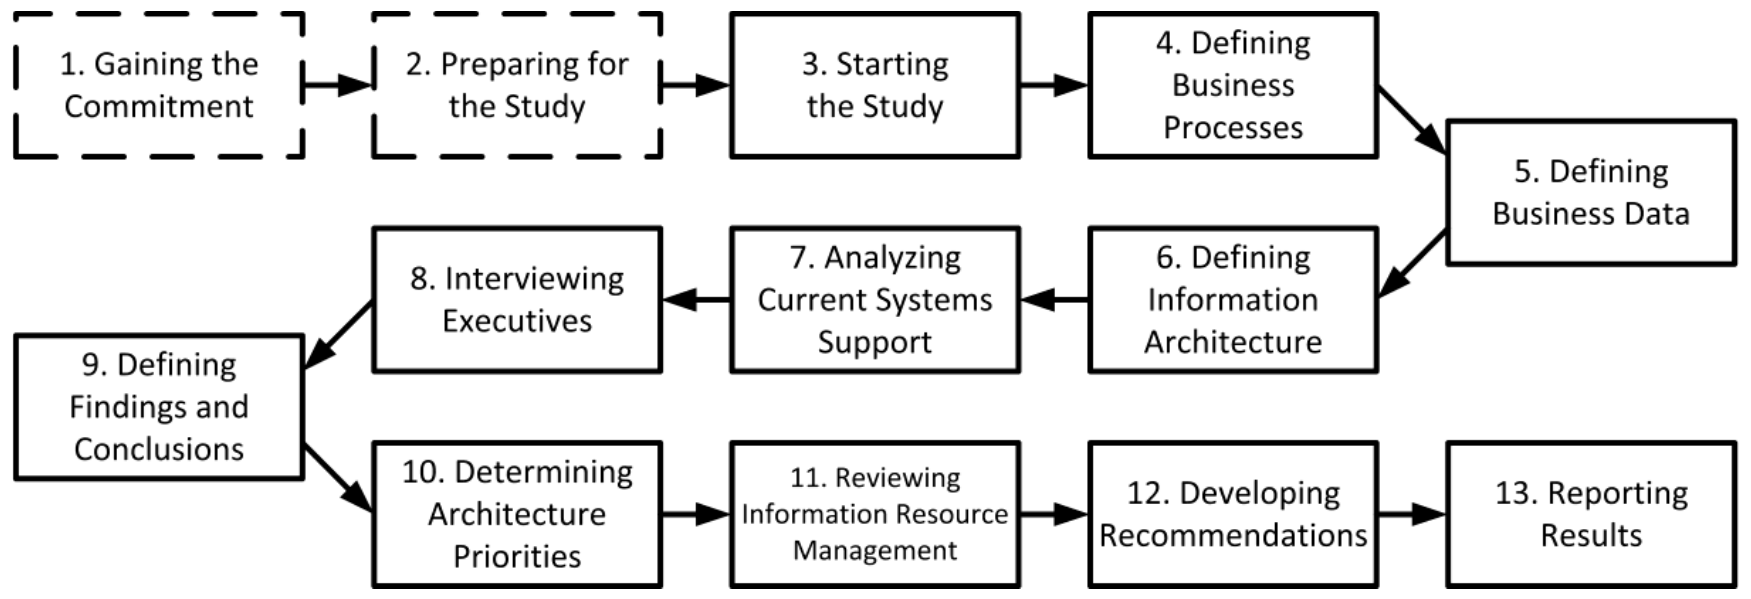
\includegraphics[width=\textwidth]{../figures/bsp}
			\end{center}
		\end{frame}
	}

	\begin{frame}
		\frametitle{Kerangka Kerja Arsitektur PRISM}
		\begin{itemize}
			\item Salah satu kerangka kerja arsitektur perusahaan pertama
			\item Dikembangkan oleh konsorsium vendor IT
			\item Berfokus pada integrasi sistem dan teknologi informasi
			\item Membantu organisasi untuk memahami dan mengatur kompleksitas TI
		\end{itemize}
	\end{frame}
	
	{
		\setbeamertemplate{navigation symbols}{}
		\setbeamertemplate{footline}{}		
		\begin{frame}
			\frametitle{PRISM Enterprise Architecture Framework}
			\begin{center}
				
				\begin{figure}[ht]
					\begin{minipage}[b]{0.49\linewidth}
						\centering
						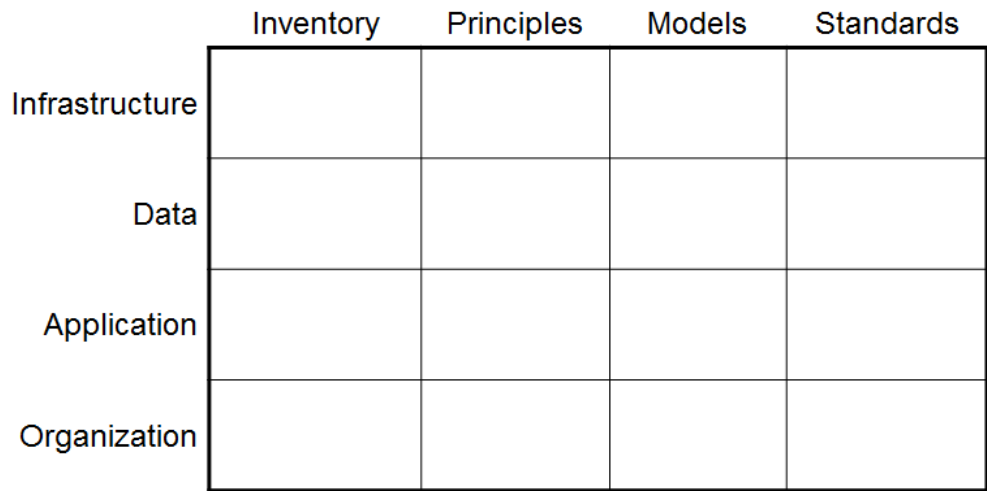
\includegraphics[width=\textwidth]{../figures/prism_matrix}
						\caption{matrix}
					\end{minipage}
					\hfill
					\begin{minipage}[b]{0.49\linewidth}
						\centering
						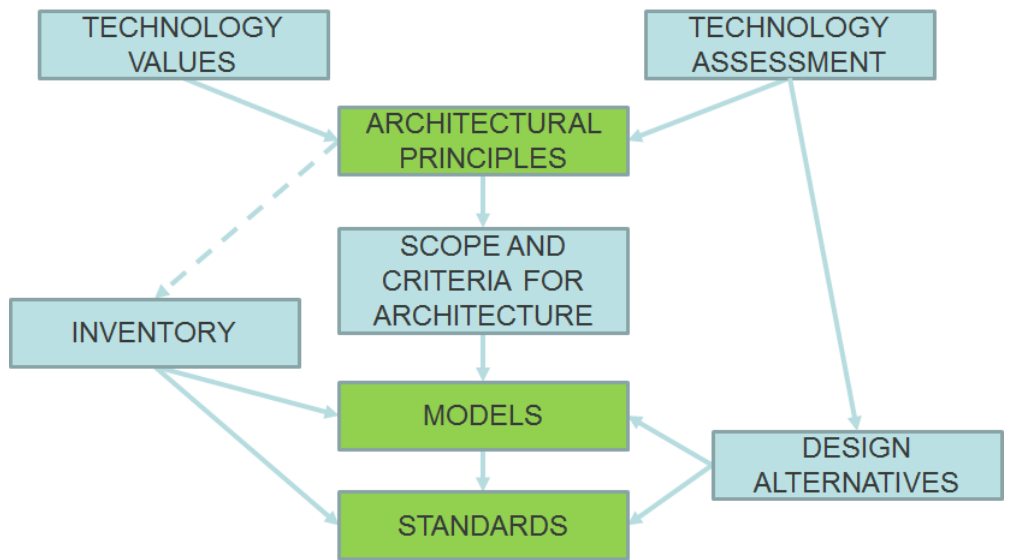
\includegraphics[width=\textwidth]{../figures/prism_relationships}
						\caption{relationships}
					\end{minipage}
				\end{figure}
				
			\end{center}
		\end{frame}
	}

	\begin{frame}
		\frametitle{Model Arsitektur Perusahaan NIST}
		\begin{itemize}
			\item Menekankan strukturisasi dan pengorganisasian operasi IT
			\item Membagi arsitektur IT menjadi lima tingkatan
			\item Berfokus pada bisnis, data, aplikasi, teknologi, dan hasil
			\item Memungkinkan perencanaan strategis dan pengambilan keputusan berdasarkan data
		\end{itemize}
	\end{frame}

	{
		\setbeamertemplate{navigation symbols}{}
		\setbeamertemplate{footline}{}		
		\begin{frame}
			\frametitle{NIST Enterprise Architecture Framework}
			\begin{center}
				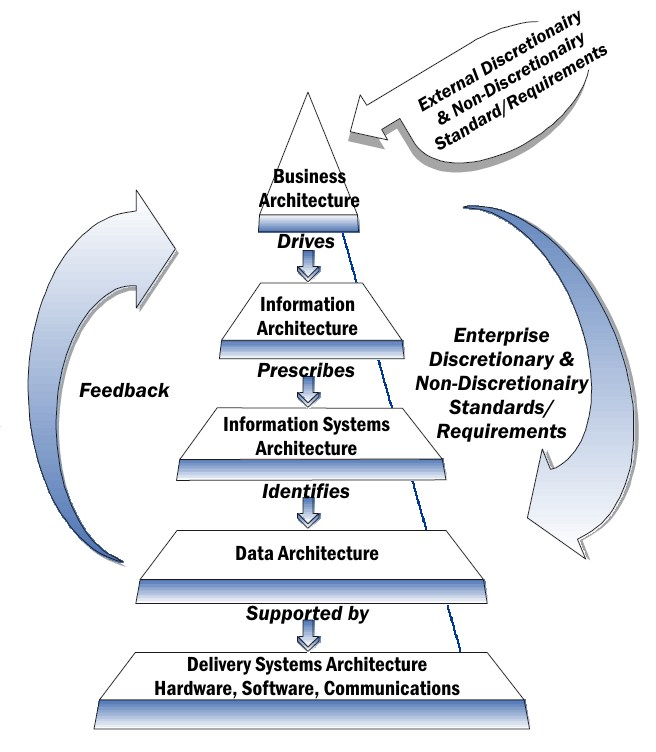
\includegraphics[width=.60\textwidth]{../figures/nist}
			\end{center}
		\end{frame}
	}
	
	\begin{frame}
		\frametitle{Kerangka Kerja Zachman}
		\begin{itemize}
			\item Skema untuk memahami dan mengatur kompleksitas arsitektur perusahaan
			\item Dibagi menjadi enam tingkatan berbeda
			\item Merangkum dari tingkat paling abstrak hingga paling konkret
			\item Cocok untuk berbagai jenis organisasi, dari bisnis hingga pemerintahan
		\end{itemize}
	\end{frame}
	
	{
		\setbeamertemplate{navigation symbols}{}
		\setbeamertemplate{footline}{}		
		\begin{frame}
			\frametitle{Zachman Framework}
			\begin{center}
				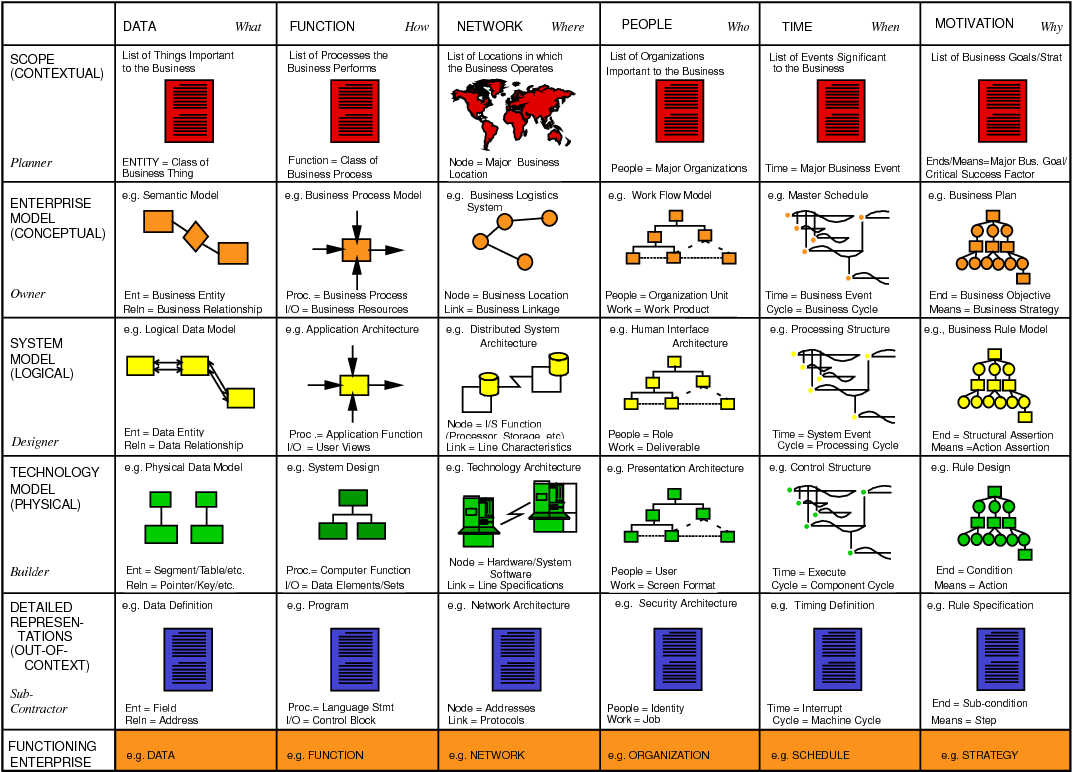
\includegraphics[width=0.9\textwidth]{../figures/zachman}
			\end{center}
		\end{frame}
	}

	\begin{frame}
		\frametitle{Perencanaan Arsitektur Perusahaan (EAP)}
		\begin{itemize}
			\item Metode untuk merencanakan arsitektur sistem informasi
			\item Mengidentifikasi apa yang dibutuhkan oleh bisnis dari teknologi informasi
			\item Menyusun rencana untuk implementasi teknologi baru berdasarkan kebutuhan bisnis
			\item Dapat membantu dalam transformasi digital dan perubahan organisasi
		\end{itemize}
	\end{frame}
	
	{
		\setbeamertemplate{navigation symbols}{}
		\setbeamertemplate{footline}{}		
		\begin{frame}
			\frametitle{Enterprise Architecture Planning}
			\begin{center}
				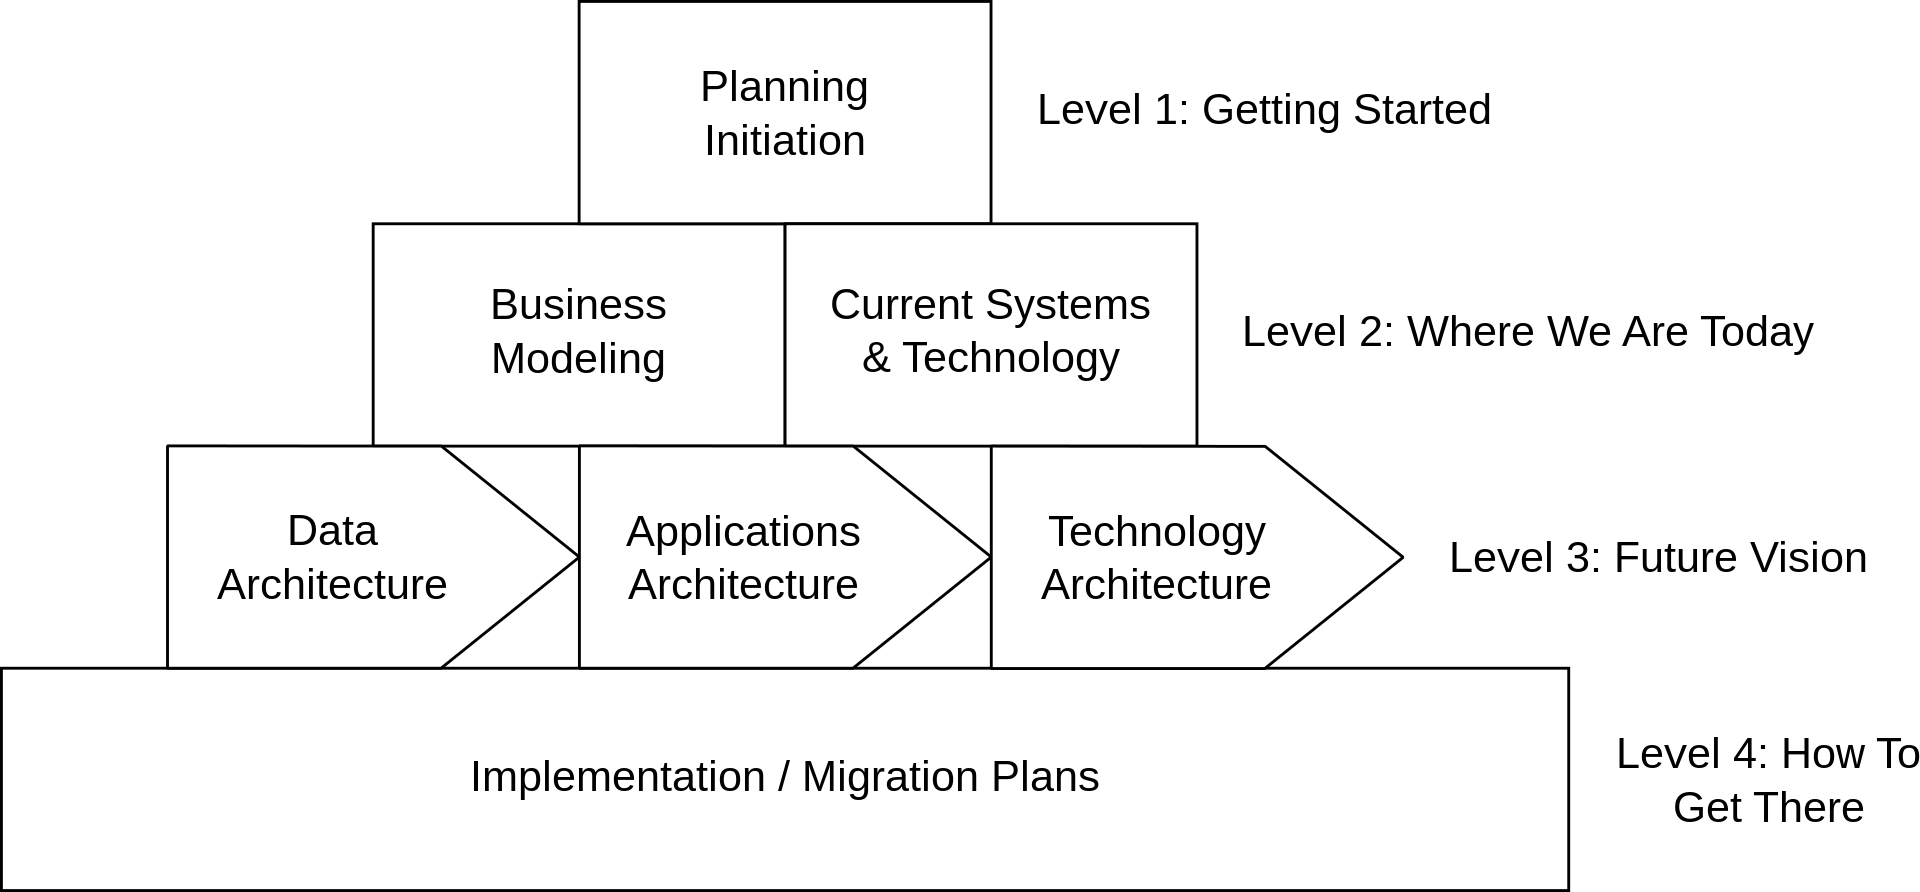
\includegraphics[width=1\textwidth]{../figures/eap}
			\end{center}
		\end{frame}
	}

	\begin{frame}
		\frametitle{Arsitektur Keamanan Bisnis Terapan Sherwood (SABSA)}
		\begin{itemize}
			\item Model dan metodologi untuk mengembangkan kerangka kerja keamanan informasi dan manajemen risiko
			\item Merancang, mengimplementasikan, dan mengelola solusi keamanan yang berpusat pada bisnis
			\item Dikembangkan dengan pendekatan "awal-hingga-akhir" dan "atas-ke-bawah"
			\item Dapat disesuaikan dengan kebutuhan spesifik organisasi
		\end{itemize}
	\end{frame}
	
	{
		\setbeamertemplate{navigation symbols}{}
		\setbeamertemplate{footline}{}		
		\begin{frame}
			\frametitle{Sherwood Applied Business Security Architecture (SABSA)}
			\begin{center}
				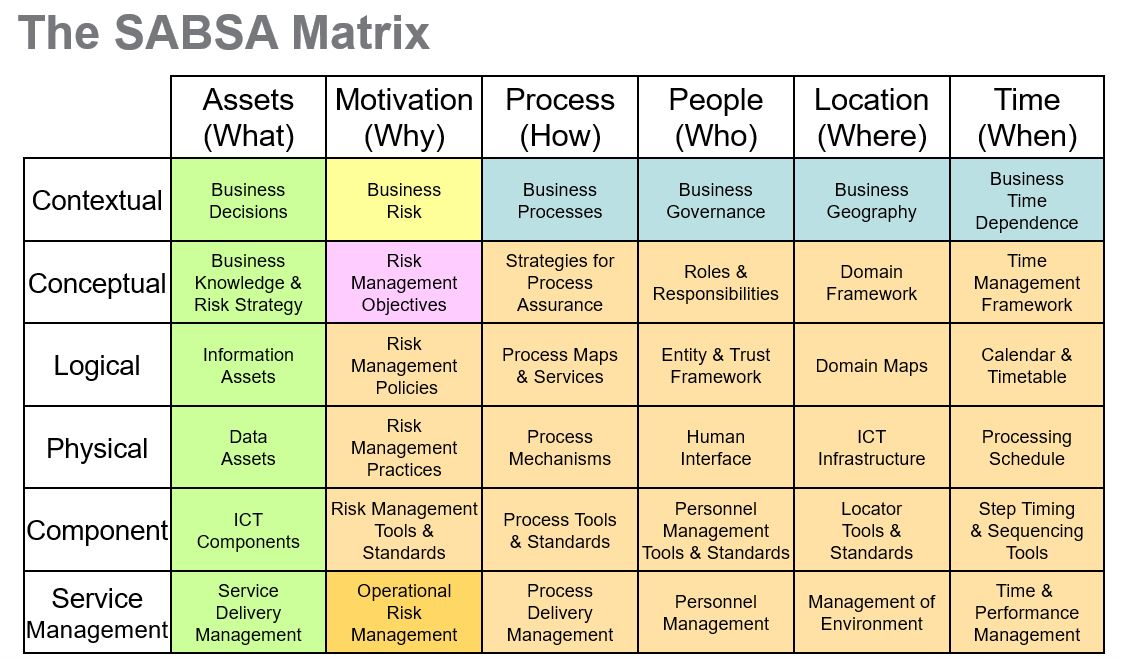
\includegraphics[width=1\textwidth]{../figures/sabsa}
			\end{center}
		\end{frame}
	}

	
	\begin{frame}
		\frametitle{Federal Enterprise Architecture Framework (FEAF)}
		\begin{itemize}
			\item Kerangka kerja yang digunakan oleh pemerintah federal AS
			\item Membantu dalam meningkatkan efisiensi dan efektivitas pelayanan pemerintah
			\item Memfasilitasi kerjasama antar agen dan departemen pemerintah
			\item Merupakan bagian dari strategi modernisasi teknologi informasi pemerintah AS
		\end{itemize}
	\end{frame}
	
	{
		\setbeamertemplate{navigation symbols}{}
		\setbeamertemplate{footline}{}		
		\begin{frame}
			\frametitle{Federal Enterprsie Architecture Framework}
			\begin{center}
				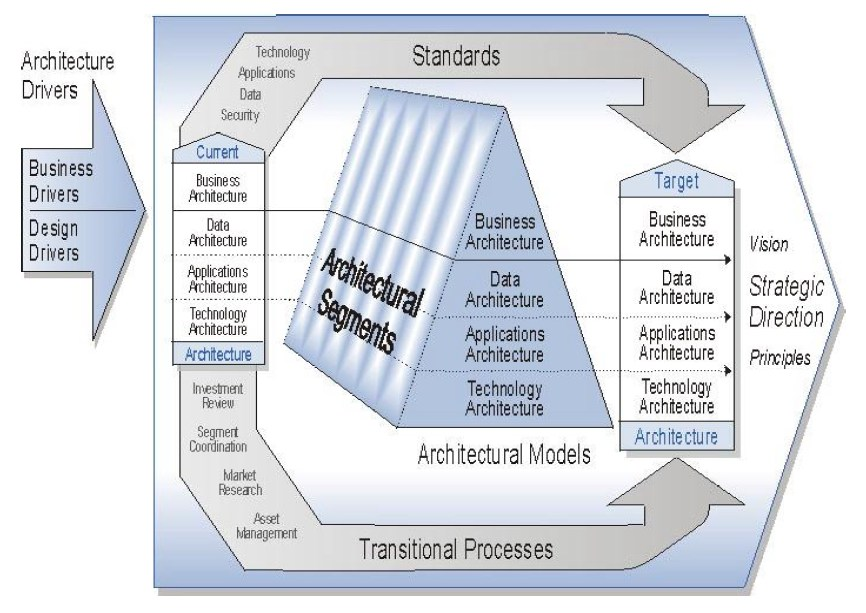
\includegraphics[width=.95\textwidth]{../figures/feaf}
			\end{center}
		\end{frame}
	}

	\begin{frame}
		\frametitle{Metode Arsitektur Perusahaan Gartner}
		\begin{itemize}
			\item Metode yang dikembangkan oleh perusahaan riset dan konsultasi Gartner
			\item Memandu organisasi dalam merancang, mengembangkan, dan mengimplementasikan arsitektur perusahaan
			\item Menghubungkan strategi bisnis dan IT
			\item Membantu organisasi dalam mencapai tujuan transformasi digital
		\end{itemize}
	\end{frame}
	
	{
		\setbeamertemplate{navigation symbols}{}
		\setbeamertemplate{footline}{}		
		\begin{frame}
			\frametitle{Gartner's Enterprise Architecture Process}
			\begin{center}
				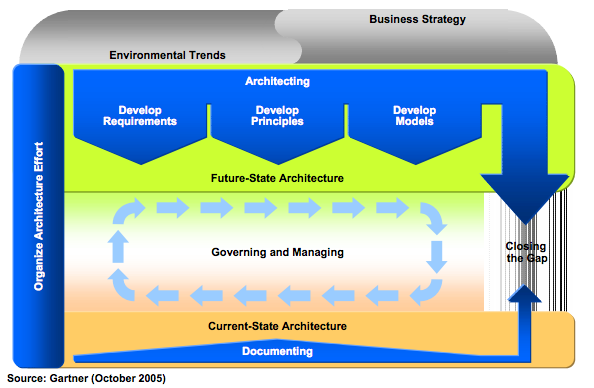
\includegraphics[width=.95\textwidth]{../figures/gartner}
			\end{center}
		\end{frame}
	}

	\begin{frame}
		\frametitle{Kerangka Kerja Arsitektur Departemen Pertahanan (DoDAF)}
		\begin{itemize}
			\item Kerangka kerja yang digunakan oleh Departemen Pertahanan AS
			\item Membantu dalam mengorganisasi dan memvisualisasikan informasi yang penting untuk proses pengambilan keputusan
			\item Menggunakan berbagai model dan panduan untuk mengembangkan arsitektur
			\item Cocok untuk organisasi dengan kompleksitas dan skala besar
		\end{itemize}
	\end{frame}
	
	{
		\setbeamertemplate{navigation symbols}{}
		\setbeamertemplate{footline}{}		
		\begin{frame}
			\frametitle{Department of Defence Architecture Framework (DoDAF)}
			\begin{center}
				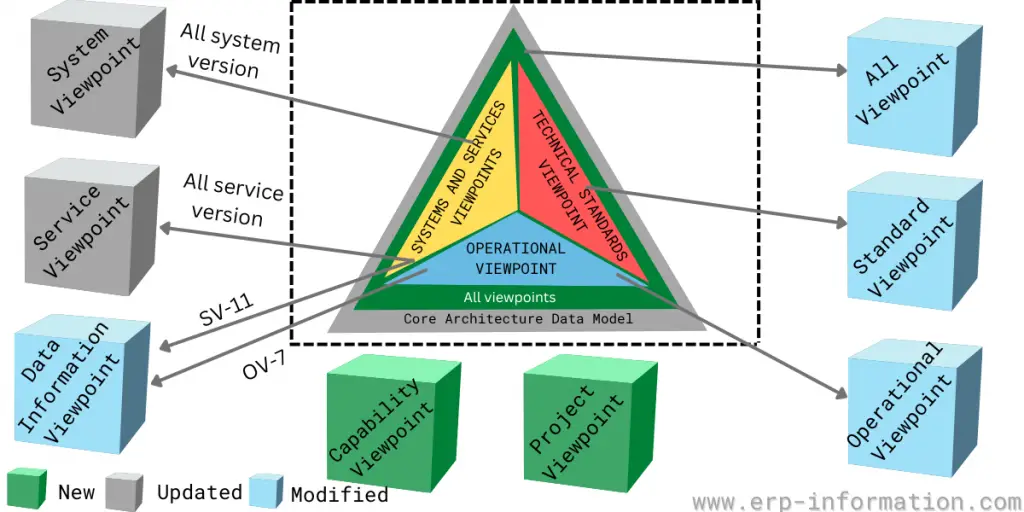
\includegraphics[width=0.9\textwidth]{../figures/dodaf}
			\end{center}
		\end{frame}
	}

	\begin{frame}
		\frametitle{Pemerintah Australia AGA}
		\begin{itemize}
			\item Kerangka kerja yang digunakan oleh Pemerintah Australia
			\item Membantu dalam perencanaan dan implementasi teknologi informasi di tingkat pemerintahan
			\item Mendorong kolaborasi antar departemen dan agen pemerintah
			\item Meningkatkan efisiensi dan transparansi dalam layanan pemerintah
		\end{itemize}
	\end{frame}
	
	{
		\setbeamertemplate{navigation symbols}{}
		\setbeamertemplate{footline}{}		
		\begin{frame}
			\frametitle{Austarlian Government Architecture (AGA)}
			\begin{center}
				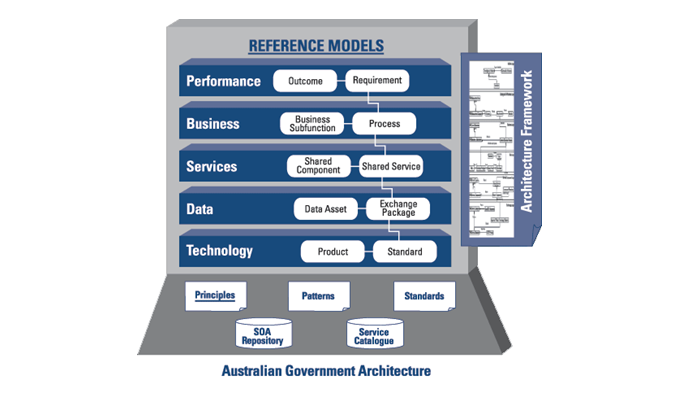
\includegraphics[width=1.1\textwidth]{../figures/aga}
			\end{center}
		\end{frame}
	}
	
	\begin{frame}
		\frametitle{Body of Knowledge Arsitektur Bisnis (BizBoK)}
		\begin{itemize}
			\item Panduan yang dikembangkan oleh Business Architecture Guild
			\item Menyediakan praktik terbaik dan standar dalam arsitektur bisnis
			\item Dapat digunakan oleh arsitek bisnis dan profesional terkait lainnya
			\item Membantu organisasi dalam merancang dan mengimplementasikan arsitektur bisnis
		\end{itemize}
	\end{frame}
	
		{
		\setbeamertemplate{navigation symbols}{}
		\setbeamertemplate{footline}{}		
		\begin{frame}
			\frametitle{Business Architecture Body Of Knowledge}
			\begin{center}
				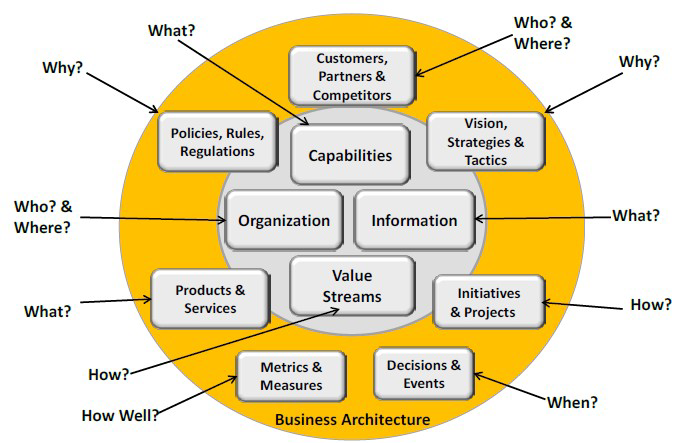
\includegraphics[width=1\textwidth]{../figures/bizbok}
			\end{center}
		\end{frame}
	}

	\begin{frame}
		\frametitle{Standar ISO untuk Pemodelan Perusahaan (ISO19439)}
		\begin{itemize}
			\item Standar internasional untuk pemodelan proses bisnis dan organisasi
			\item Membantu dalam perencanaan, desain, dan perbaikan proses bisnis
			\item Dapat digunakan oleh berbagai jenis organisasi, dari bisnis hingga pemerintahan
			\item Dikembangkan oleh Organisasi Internasional untuk Standardisasi (ISO)
		\end{itemize}
	\end{frame}
	
	{
		\setbeamertemplate{navigation symbols}{}
		\setbeamertemplate{footline}{}		
		\begin{frame}
			\frametitle{ISO19439 Enterprise Modelling}
			\begin{center}
				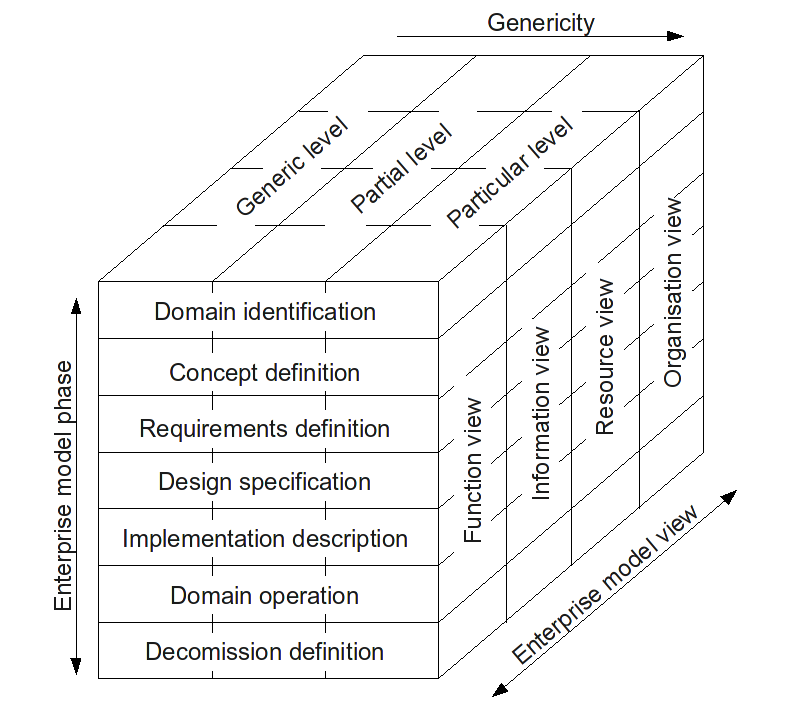
\includegraphics[width=.75\textwidth]{../figures/iso19439}
			\end{center}
		\end{frame}
	}

	\begin{frame}
		\frametitle{Ringkasan}
		\begin{itemize}
			\item Ada berbagai kerangka kerja dan metodologi arsitektur perusahaan
			\item Pilihan kerangka kerja atau metodologi tergantung pada kebutuhan dan konteks spesifik organisasi
			\item Arsitektur perusahaan adalah alat penting untuk merencanakan dan mengelola teknologi informasi di organisasi
		\end{itemize}
	\end{frame}

\end{document}